% Options for packages loaded elsewhere
\PassOptionsToPackage{unicode}{hyperref}
\PassOptionsToPackage{hyphens}{url}
%
\documentclass[
]{article}
\usepackage{amsmath,amssymb}
\usepackage{lmodern}
\usepackage{ifxetex,ifluatex}
\ifnum 0\ifxetex 1\fi\ifluatex 1\fi=0 % if pdftex
  \usepackage[T1]{fontenc}
  \usepackage[utf8]{inputenc}
  \usepackage{textcomp} % provide euro and other symbols
\else % if luatex or xetex
  \usepackage{unicode-math}
  \defaultfontfeatures{Scale=MatchLowercase}
  \defaultfontfeatures[\rmfamily]{Ligatures=TeX,Scale=1}
\fi
% Use upquote if available, for straight quotes in verbatim environments
\IfFileExists{upquote.sty}{\usepackage{upquote}}{}
\IfFileExists{microtype.sty}{% use microtype if available
  \usepackage[]{microtype}
  \UseMicrotypeSet[protrusion]{basicmath} % disable protrusion for tt fonts
}{}
\makeatletter
\@ifundefined{KOMAClassName}{% if non-KOMA class
  \IfFileExists{parskip.sty}{%
    \usepackage{parskip}
  }{% else
    \setlength{\parindent}{0pt}
    \setlength{\parskip}{6pt plus 2pt minus 1pt}}
}{% if KOMA class
  \KOMAoptions{parskip=half}}
\makeatother
\usepackage{xcolor}
\IfFileExists{xurl.sty}{\usepackage{xurl}}{} % add URL line breaks if available
\IfFileExists{bookmark.sty}{\usepackage{bookmark}}{\usepackage{hyperref}}
\hypersetup{
  pdftitle={Assignment2Notebook},
  pdfauthor={Fengfan},
  hidelinks,
  pdfcreator={LaTeX via pandoc}}
\urlstyle{same} % disable monospaced font for URLs
\usepackage[margin=1in]{geometry}
\usepackage{color}
\usepackage{fancyvrb}
\newcommand{\VerbBar}{|}
\newcommand{\VERB}{\Verb[commandchars=\\\{\}]}
\DefineVerbatimEnvironment{Highlighting}{Verbatim}{commandchars=\\\{\}}
% Add ',fontsize=\small' for more characters per line
\usepackage{framed}
\definecolor{shadecolor}{RGB}{248,248,248}
\newenvironment{Shaded}{\begin{snugshade}}{\end{snugshade}}
\newcommand{\AlertTok}[1]{\textcolor[rgb]{0.94,0.16,0.16}{#1}}
\newcommand{\AnnotationTok}[1]{\textcolor[rgb]{0.56,0.35,0.01}{\textbf{\textit{#1}}}}
\newcommand{\AttributeTok}[1]{\textcolor[rgb]{0.77,0.63,0.00}{#1}}
\newcommand{\BaseNTok}[1]{\textcolor[rgb]{0.00,0.00,0.81}{#1}}
\newcommand{\BuiltInTok}[1]{#1}
\newcommand{\CharTok}[1]{\textcolor[rgb]{0.31,0.60,0.02}{#1}}
\newcommand{\CommentTok}[1]{\textcolor[rgb]{0.56,0.35,0.01}{\textit{#1}}}
\newcommand{\CommentVarTok}[1]{\textcolor[rgb]{0.56,0.35,0.01}{\textbf{\textit{#1}}}}
\newcommand{\ConstantTok}[1]{\textcolor[rgb]{0.00,0.00,0.00}{#1}}
\newcommand{\ControlFlowTok}[1]{\textcolor[rgb]{0.13,0.29,0.53}{\textbf{#1}}}
\newcommand{\DataTypeTok}[1]{\textcolor[rgb]{0.13,0.29,0.53}{#1}}
\newcommand{\DecValTok}[1]{\textcolor[rgb]{0.00,0.00,0.81}{#1}}
\newcommand{\DocumentationTok}[1]{\textcolor[rgb]{0.56,0.35,0.01}{\textbf{\textit{#1}}}}
\newcommand{\ErrorTok}[1]{\textcolor[rgb]{0.64,0.00,0.00}{\textbf{#1}}}
\newcommand{\ExtensionTok}[1]{#1}
\newcommand{\FloatTok}[1]{\textcolor[rgb]{0.00,0.00,0.81}{#1}}
\newcommand{\FunctionTok}[1]{\textcolor[rgb]{0.00,0.00,0.00}{#1}}
\newcommand{\ImportTok}[1]{#1}
\newcommand{\InformationTok}[1]{\textcolor[rgb]{0.56,0.35,0.01}{\textbf{\textit{#1}}}}
\newcommand{\KeywordTok}[1]{\textcolor[rgb]{0.13,0.29,0.53}{\textbf{#1}}}
\newcommand{\NormalTok}[1]{#1}
\newcommand{\OperatorTok}[1]{\textcolor[rgb]{0.81,0.36,0.00}{\textbf{#1}}}
\newcommand{\OtherTok}[1]{\textcolor[rgb]{0.56,0.35,0.01}{#1}}
\newcommand{\PreprocessorTok}[1]{\textcolor[rgb]{0.56,0.35,0.01}{\textit{#1}}}
\newcommand{\RegionMarkerTok}[1]{#1}
\newcommand{\SpecialCharTok}[1]{\textcolor[rgb]{0.00,0.00,0.00}{#1}}
\newcommand{\SpecialStringTok}[1]{\textcolor[rgb]{0.31,0.60,0.02}{#1}}
\newcommand{\StringTok}[1]{\textcolor[rgb]{0.31,0.60,0.02}{#1}}
\newcommand{\VariableTok}[1]{\textcolor[rgb]{0.00,0.00,0.00}{#1}}
\newcommand{\VerbatimStringTok}[1]{\textcolor[rgb]{0.31,0.60,0.02}{#1}}
\newcommand{\WarningTok}[1]{\textcolor[rgb]{0.56,0.35,0.01}{\textbf{\textit{#1}}}}
\usepackage{graphicx}
\makeatletter
\def\maxwidth{\ifdim\Gin@nat@width>\linewidth\linewidth\else\Gin@nat@width\fi}
\def\maxheight{\ifdim\Gin@nat@height>\textheight\textheight\else\Gin@nat@height\fi}
\makeatother
% Scale images if necessary, so that they will not overflow the page
% margins by default, and it is still possible to overwrite the defaults
% using explicit options in \includegraphics[width, height, ...]{}
\setkeys{Gin}{width=\maxwidth,height=\maxheight,keepaspectratio}
% Set default figure placement to htbp
\makeatletter
\def\fps@figure{htbp}
\makeatother
\setlength{\emergencystretch}{3em} % prevent overfull lines
\providecommand{\tightlist}{%
  \setlength{\itemsep}{0pt}\setlength{\parskip}{0pt}}
\setcounter{secnumdepth}{-\maxdimen} % remove section numbering
\ifluatex
  \usepackage{selnolig}  % disable illegal ligatures
\fi

\title{Assignment2Notebook}
\author{Fengfan}
\date{07/10/2021}

\begin{document}
\maketitle

\hypertarget{packages}{%
\subsection{Packages}\label{packages}}

\textbf{Install \emph{Tidyverse} }
\texttt{install.packages("tidyverse")}\\
Tidyverse library is a superset of \texttt{ggplot2} library

\textbf{Load library}

\begin{Shaded}
\begin{Highlighting}[]
\FunctionTok{library}\NormalTok{(tidyverse)}
\end{Highlighting}
\end{Shaded}

\begin{verbatim}
## -- Attaching packages --------------------------------------- tidyverse 1.3.1 --
\end{verbatim}

\begin{verbatim}
## v ggplot2 3.3.5     v purrr   0.3.4
## v tibble  3.1.5     v dplyr   1.0.7
## v tidyr   1.1.4     v stringr 1.4.0
## v readr   2.0.2     v forcats 0.5.1
\end{verbatim}

\begin{verbatim}
## -- Conflicts ------------------------------------------ tidyverse_conflicts() --
## x dplyr::filter() masks stats::filter()
## x dplyr::lag()    masks stats::lag()
\end{verbatim}

\textbf{Load Data from packages} \texttt{Stat2Data} package contains
information about 908 Hawks \texttt{install.packages("Stat2Data")}

\begin{Shaded}
\begin{Highlighting}[]
\FunctionTok{library}\NormalTok{(Stat2Data)}
\FunctionTok{data}\NormalTok{(}\StringTok{"Hawks"}\NormalTok{)}

\CommentTok{\# Load data from the packages}
\NormalTok{hawksSmall}\OtherTok{\textless{}{-}}\FunctionTok{drop\_na}\NormalTok{(}\FunctionTok{select}\NormalTok{(Hawks,Age,Day,Month,Year,CaptureTime,Species,Wing,Weight,Tail))}

\FunctionTok{head}\NormalTok{(hawksSmall)}
\end{Highlighting}
\end{Shaded}

\begin{verbatim}
##   Age Day Month Year CaptureTime Species Wing Weight Tail
## 1   I  19     9 1992       13:30      RT  385    920  219
## 2   I  22     9 1992       10:30      RT  376    930  221
## 3   I  23     9 1992       12:45      RT  381    990  235
## 4   I  23     9 1992       10:50      CH  265    470  220
## 5   I  27     9 1992       11:15      SS  205    170  157
## 6   I  28     9 1992       11:25      RT  412   1090  230
\end{verbatim}

\hypertarget{type-of-variables}{%
\subsubsection{1.1 Type of Variables}\label{type-of-variables}}

\texttt{dim()} is used to show the rows of the data.\\
And \texttt{head()} is used to show the first 5 rows of the data.

\begin{Shaded}
\begin{Highlighting}[]
\FunctionTok{dim}\NormalTok{(hawksSmall)}
\end{Highlighting}
\end{Shaded}

\begin{verbatim}
## [1] 897   9
\end{verbatim}

It shows that the data have 897 rows and 9 columns.

\begin{Shaded}
\begin{Highlighting}[]
\FunctionTok{mode}\NormalTok{(hawksSmall)}
\end{Highlighting}
\end{Shaded}

\begin{verbatim}
## [1] "list"
\end{verbatim}

For each of the following variables say whether they continuous,
discrete or categorical. Discuss this with your colleagues.

\begin{enumerate}
\def\labelenumi{\arabic{enumi}.}
\tightlist
\item
  Month -\textgreater{} Categorical\\
\item
  Species -\textgreater{} Categorical\\
\item
  Age -\textgreater{} Discrete\\
\item
  Wing -\textgreater{} Discrete\\
\item
  Weight -\textgreater{} Continous
\end{enumerate}

\begin{center}\rule{0.5\linewidth}{0.5pt}\end{center}

\hypertarget{whats-wrong-with-this-plot}{%
\subsubsection{1.2 What's wrong with this
plot?}\label{whats-wrong-with-this-plot}}

Write down some problems with the plot displayed below.

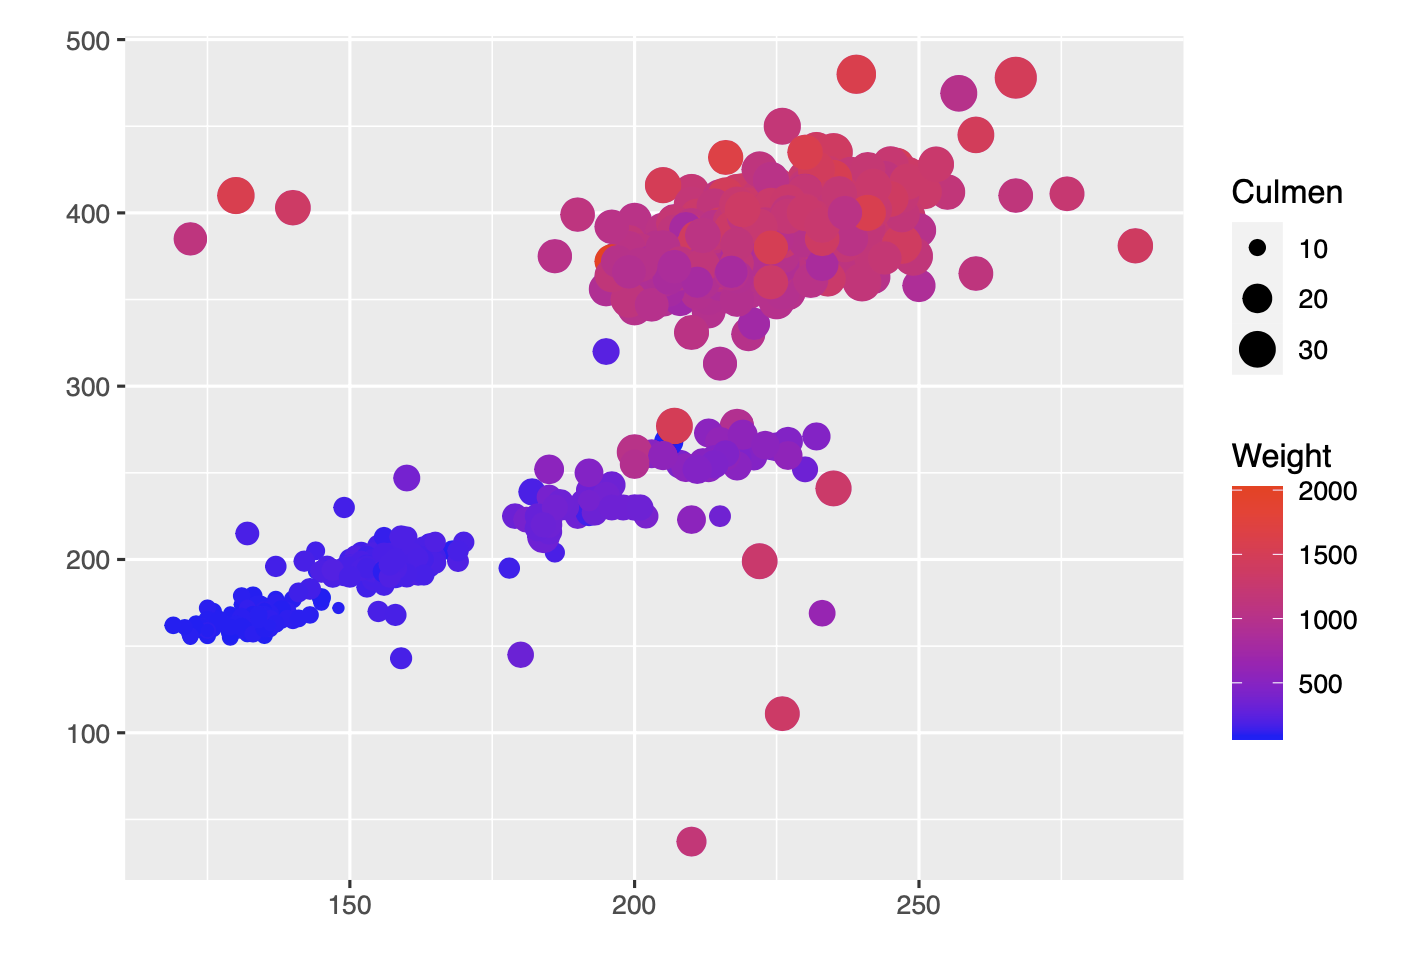
\includegraphics{/Users/frankhu/Documents/SCEM/firstRProject/img/2-1.2.png}

\textbf{Problems}\\
1. It doesn't show the name of the X and Y axes.\\
2. The value of weight varies from 0 to 2000, the range is too big which
cause the size range big.

\hypertarget{generate-a-histogram}{%
\subsubsection{1.3 Generate a histogram}\label{generate-a-histogram}}

Next use a combination of the functions \texttt{ggplot()} and
geom\_histogram to create a histogram plot of the weights of the Hawks
within the hawksSmall data frame with bin widths of 100 grams. Your
result should look something like this:

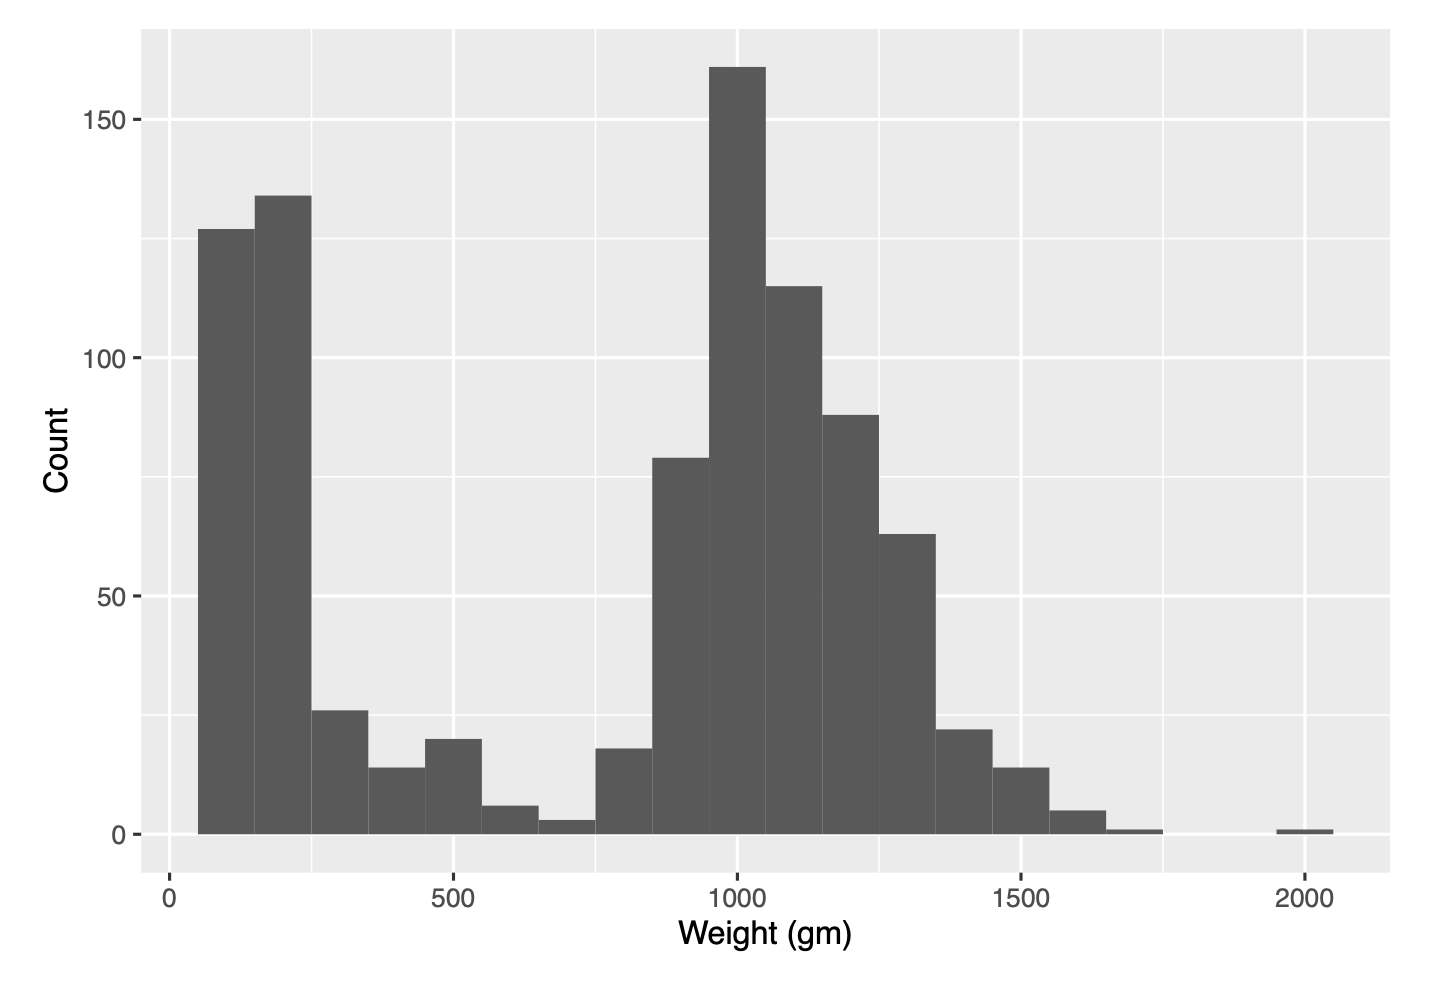
\includegraphics{/Users/frankhu/Documents/SCEM/firstRProject/img/2-1.3.png}
Codes here:

\begin{Shaded}
\begin{Highlighting}[]
\CommentTok{\# aes() are used to draw selected features of the data.}
\CommentTok{\# Assign the binwidth argument to specify the binwidth of the histogram.}
\NormalTok{hawks\_histogram }\OtherTok{\textless{}{-}} \FunctionTok{ggplot}\NormalTok{(hawksSmall, }\FunctionTok{aes}\NormalTok{(Weight)) }\SpecialCharTok{+} \FunctionTok{geom\_histogram}\NormalTok{(}\AttributeTok{binwidth =} \DecValTok{100}\NormalTok{)}
\CommentTok{\# Here we use labs() to rename the label.}
\NormalTok{hawks\_histogram }\SpecialCharTok{+} \FunctionTok{labs}\NormalTok{(}\AttributeTok{x=}\StringTok{"Weight (gm)"}\NormalTok{, }\AttributeTok{y=}\StringTok{"Count"}\NormalTok{)}
\end{Highlighting}
\end{Shaded}

\includegraphics{Assignment2Notebook_files/figure-latex/unnamed-chunk-5-1.pdf}

\textbf{Describe the aesthetic used within this plot}.

Weight are used in this plot.

\textbf{Which term best describes the shape of the data distribution of
Hawk weights: ``Unimodal'', ``Bimodal'' or ``Trimodal''?}

Answer: \textbf{Bimodal}

\hypertarget{generate-a-density-plot}{%
\subsubsection{1.4 Generate a density
plot}\label{generate-a-density-plot}}

Use a combination of the functions ggplot() and geom\_density() to
create a density plot of the tail lengths of the Hawks within the
hawksSmall data frame.

\begin{Shaded}
\begin{Highlighting}[]
\NormalTok{hawks\_density }\OtherTok{\textless{}{-}} \FunctionTok{ggplot}\NormalTok{(hawksSmall, }\FunctionTok{aes}\NormalTok{(Tail)) }\SpecialCharTok{+} \FunctionTok{geom\_density}\NormalTok{()}
\NormalTok{hawks\_density }\SpecialCharTok{+} \FunctionTok{labs}\NormalTok{(}\AttributeTok{x=}\StringTok{"Tail(mm)"}\NormalTok{, }\AttributeTok{y=}\StringTok{"Density"}\NormalTok{)}
\end{Highlighting}
\end{Shaded}

\includegraphics{Assignment2Notebook_files/figure-latex/unnamed-chunk-7-1.pdf}
Recreate your plot with the argument adjust = 0.5 and adjust = 1.
Describe the role played by the adjust argument within the
geom\_density() function. How many modes does the data distribution of
Hawk tail lengths have?

Answer: \textbf{3 modes}

\begin{Shaded}
\begin{Highlighting}[]
\CommentTok{\# The default value of adjust is 1, change it to 0.5}
\NormalTok{hawks\_density }\OtherTok{\textless{}{-}} \FunctionTok{ggplot}\NormalTok{(hawksSmall, }\FunctionTok{aes}\NormalTok{(Tail)) }\SpecialCharTok{+} \FunctionTok{geom\_density}\NormalTok{(}\AttributeTok{adjust=}\FloatTok{0.5}\NormalTok{)}
\NormalTok{hawks\_density }\SpecialCharTok{+} \FunctionTok{labs}\NormalTok{(}\AttributeTok{x=}\StringTok{"Tail(mm)"}\NormalTok{, }\AttributeTok{y=}\StringTok{"Density"}\NormalTok{)}
\end{Highlighting}
\end{Shaded}

\includegraphics{Assignment2Notebook_files/figure-latex/unnamed-chunk-8-1.pdf}

Create the following plots for yourself:

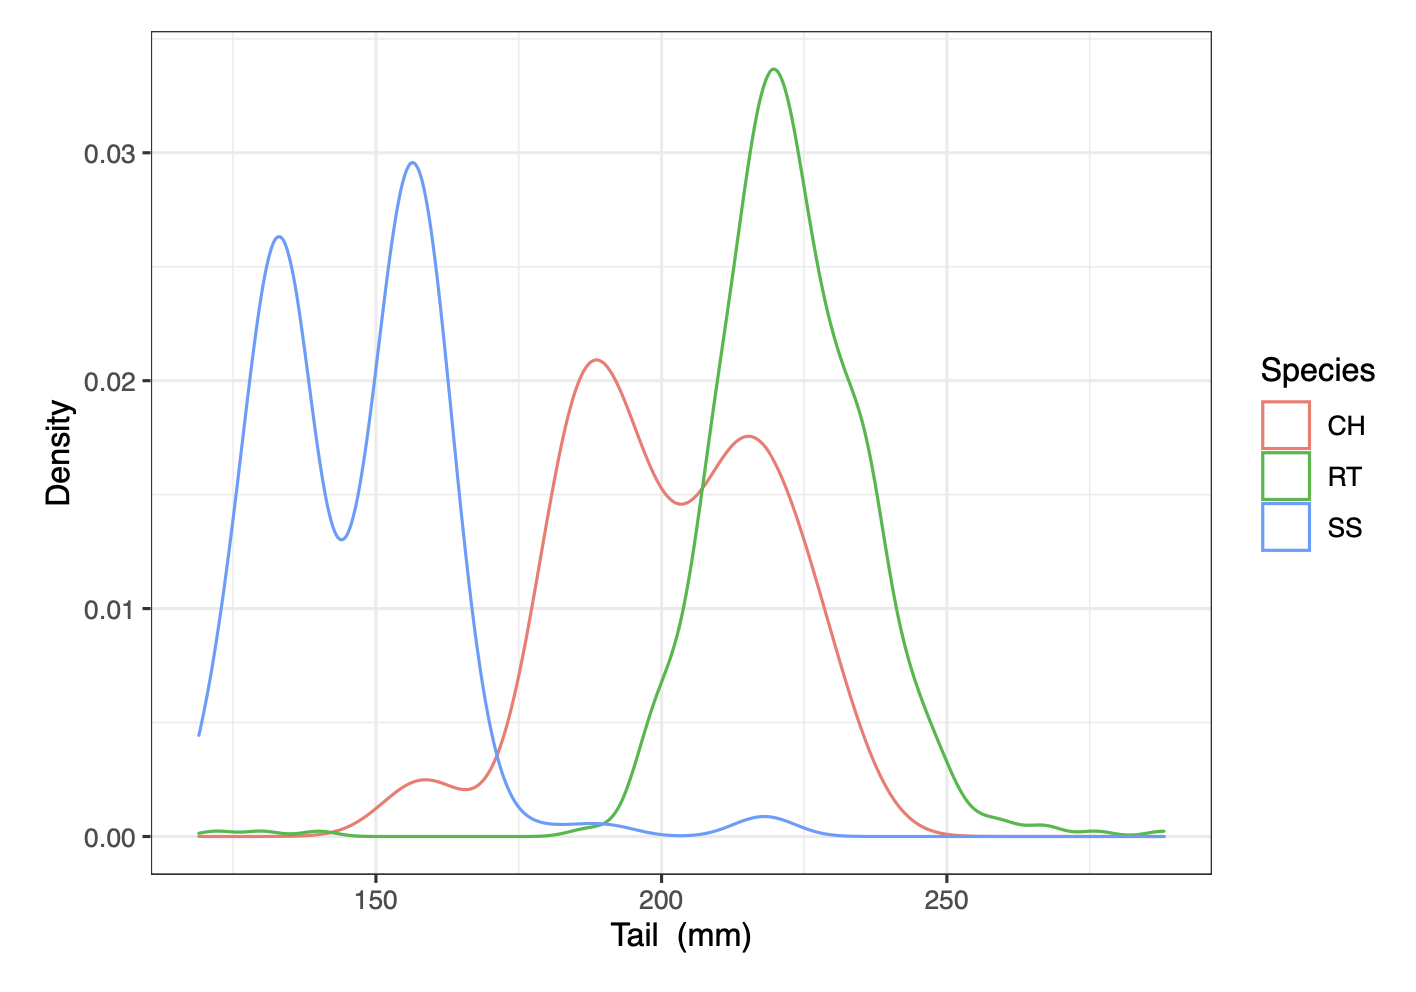
\includegraphics{/Users/frankhu/Documents/SCEM/firstRProject/img/2-1.42.png}

\begin{Shaded}
\begin{Highlighting}[]
\FunctionTok{ggplot}\NormalTok{(hawksSmall, }\FunctionTok{aes}\NormalTok{(Tail, }\AttributeTok{colour=}\NormalTok{Species)) }\SpecialCharTok{+} \FunctionTok{geom\_density}\NormalTok{() }\SpecialCharTok{+} \FunctionTok{labs}\NormalTok{(}\AttributeTok{x=}\StringTok{"Tail(mm)"}\NormalTok{, }\AttributeTok{y=}\StringTok{"Density"}\NormalTok{)}
\end{Highlighting}
\end{Shaded}

\includegraphics{Assignment2Notebook_files/figure-latex/unnamed-chunk-9-1.pdf}

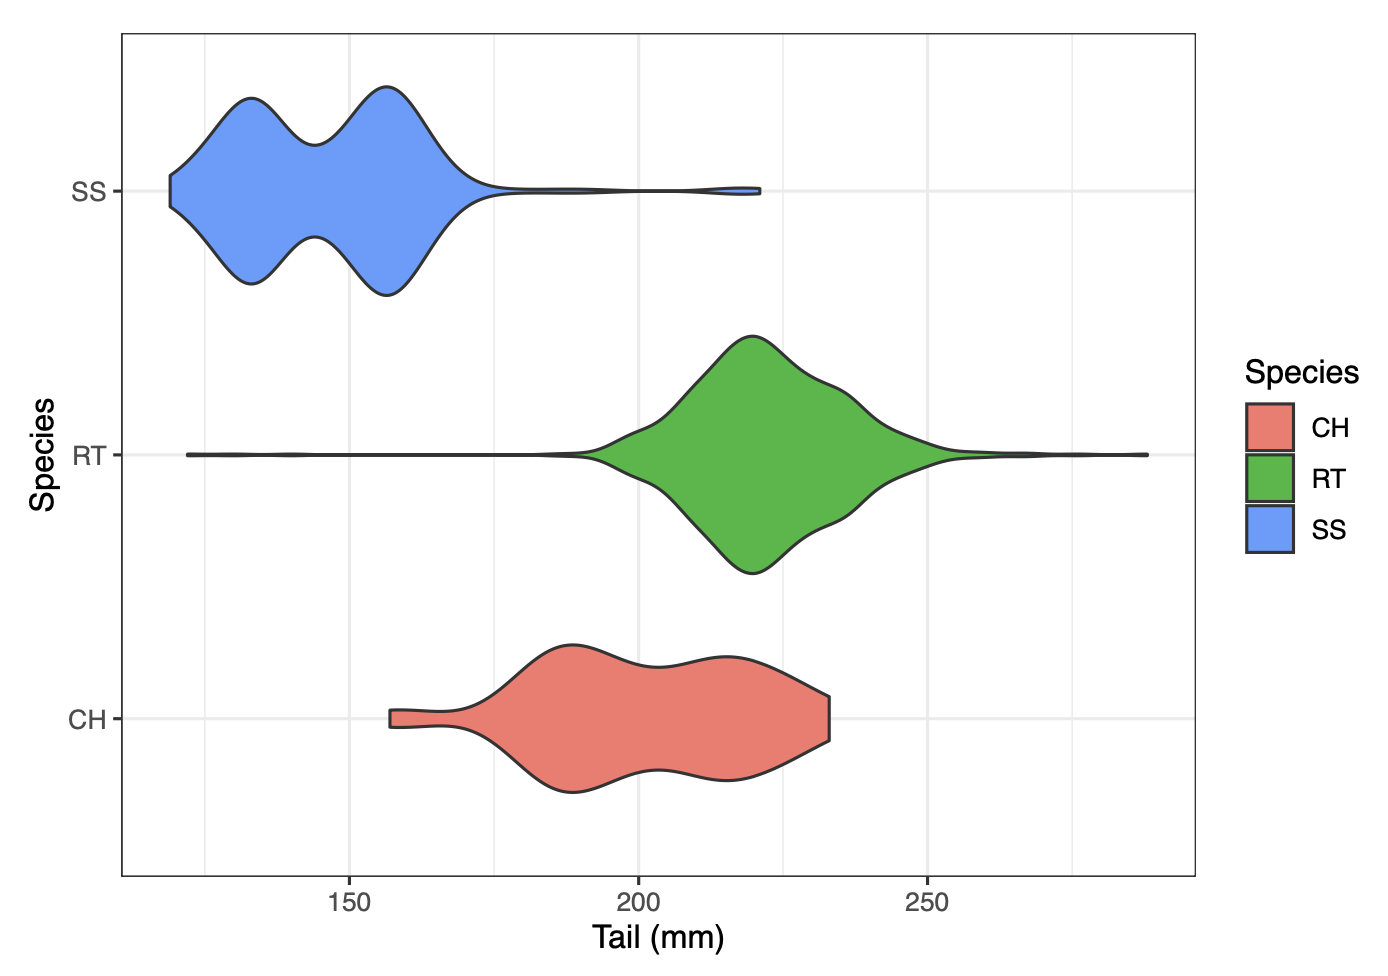
\includegraphics{/Users/frankhu/Documents/SCEM/firstRProject/img/2-1.43.png}

\begin{Shaded}
\begin{Highlighting}[]
\FunctionTok{ggplot}\NormalTok{(hawksSmall, }\FunctionTok{aes}\NormalTok{(Tail, Species, }\AttributeTok{fill=}\NormalTok{Species)) }\SpecialCharTok{+} \FunctionTok{geom\_violin}\NormalTok{() }\SpecialCharTok{+} \FunctionTok{labs}\NormalTok{(}\AttributeTok{x=}\StringTok{"Tail(mm)"}\NormalTok{, }\AttributeTok{y=}\StringTok{"Species"}\NormalTok{)}
\end{Highlighting}
\end{Shaded}

\includegraphics{Assignment2Notebook_files/figure-latex/unnamed-chunk-10-1.pdf}

\hypertarget{scatter-plots}{%
\subsubsection{1.5 Scatter plots}\label{scatter-plots}}

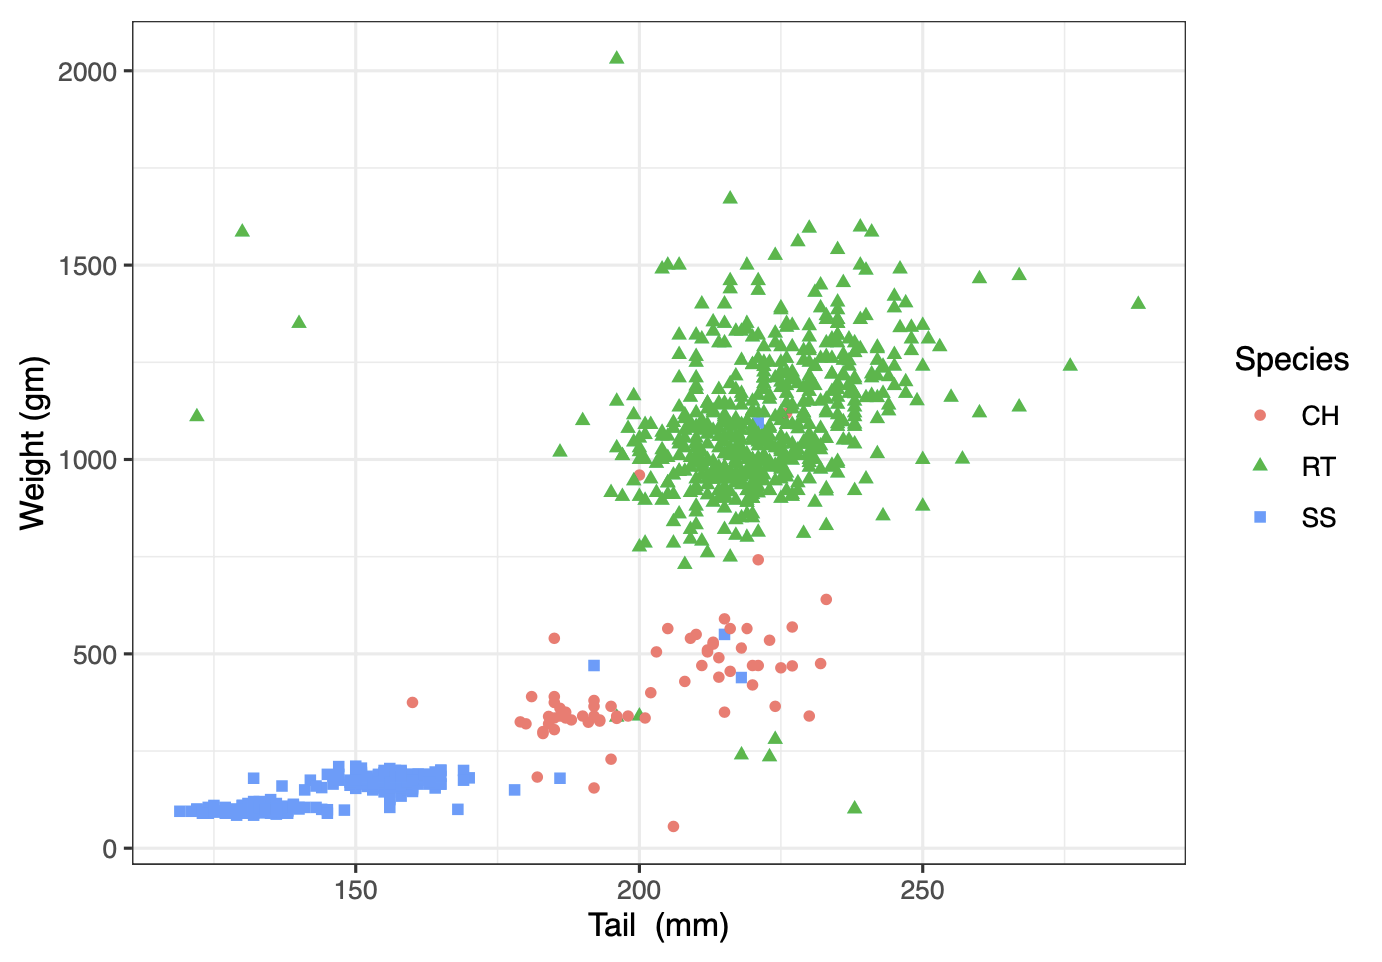
\includegraphics{/Users/frankhu/Documents/SCEM/firstRProject/img/2-1.5.png}
How many aesthetics are present within the following plot?
-\textgreater{} \textbf{X, Y, color, glyphs}\\
What are the
\href{https://en.wikipedia.org/wiki/Glyph_(data_visualization)}{glyphs}
within this plot? -\textgreater{} \textbf{Square, Circle, Triangle}

\begin{Shaded}
\begin{Highlighting}[]
\FunctionTok{ggplot}\NormalTok{(hawksSmall, }\FunctionTok{aes}\NormalTok{(Tail, Weight, }\AttributeTok{color=}\NormalTok{Species, }\AttributeTok{shape=}\NormalTok{Species)) }\SpecialCharTok{+} \FunctionTok{geom\_point}\NormalTok{()}
\end{Highlighting}
\end{Shaded}

\includegraphics{Assignment2Notebook_files/figure-latex/unnamed-chunk-11-1.pdf}

\hypertarget{trend-lines-and-facet-wraps}{%
\subsubsection{1.6 Trend lines and facet
wraps}\label{trend-lines-and-facet-wraps}}

Generate the following plot using the ggplot(), geom\_point(),
geom\_smooth() and facet\_wrap() functions.

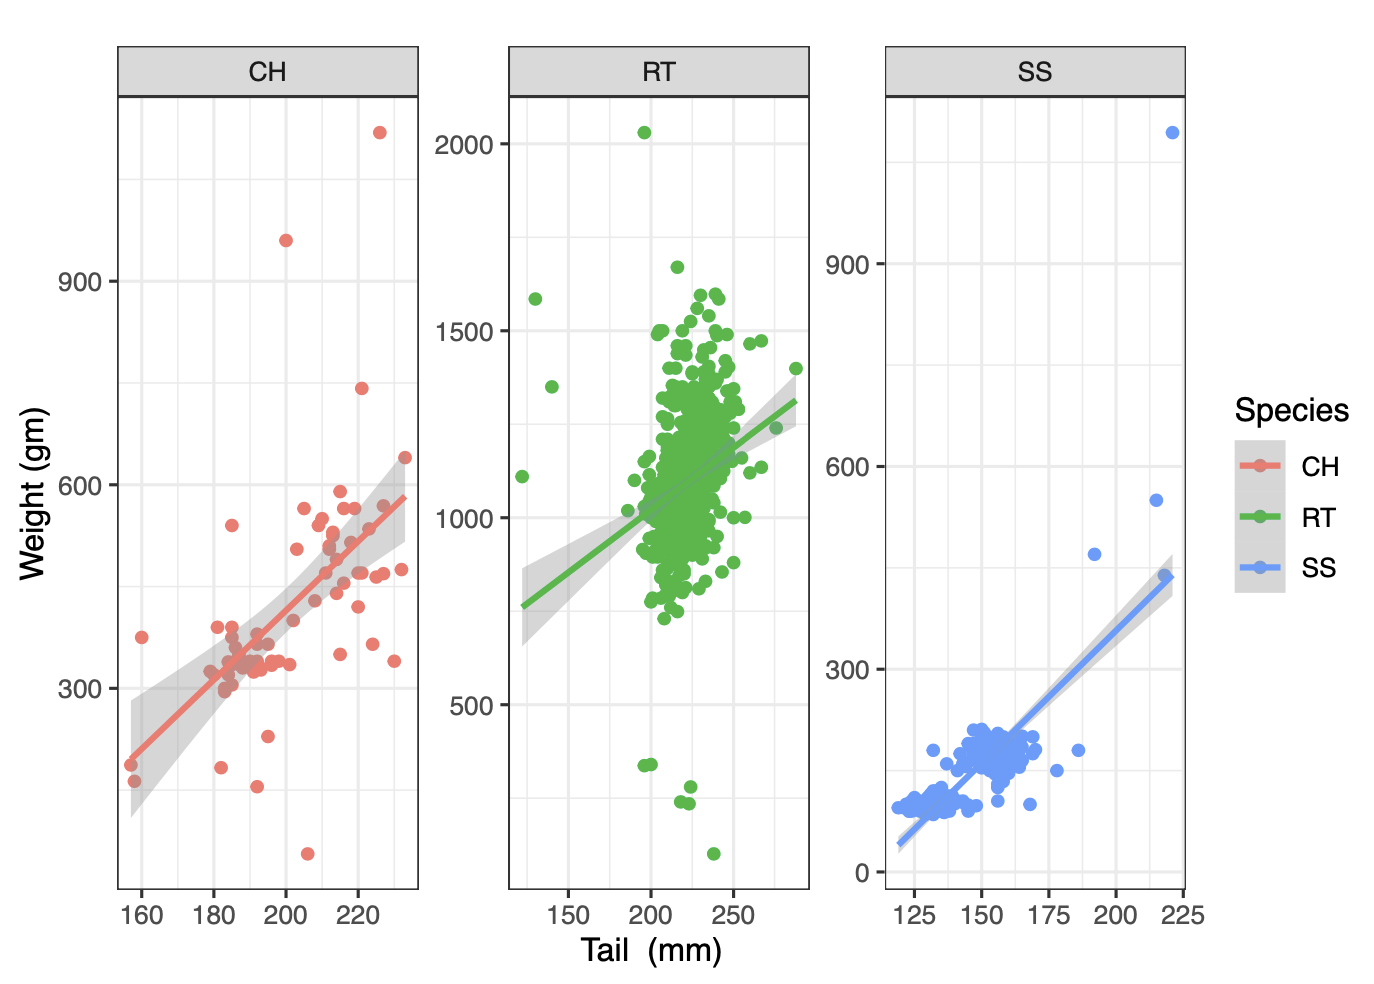
\includegraphics{/Users/frankhu/Documents/SCEM/firstRProject/img/2-1.6.png}

\begin{Shaded}
\begin{Highlighting}[]
\FunctionTok{ggplot}\NormalTok{(hawksSmall, }\FunctionTok{aes}\NormalTok{(Tail, Weight, }\AttributeTok{color=}\NormalTok{Species)) }\SpecialCharTok{+} \FunctionTok{geom\_point}\NormalTok{() }\SpecialCharTok{+} \FunctionTok{geom\_smooth}\NormalTok{(}\AttributeTok{method=}\NormalTok{lm) }\SpecialCharTok{+} \FunctionTok{facet\_wrap}\NormalTok{(}\FunctionTok{vars}\NormalTok{(Species), }\AttributeTok{scales=}\StringTok{"free"}\NormalTok{)}
\end{Highlighting}
\end{Shaded}

\begin{verbatim}
## `geom_smooth()` using formula 'y ~ x'
\end{verbatim}

\includegraphics{Assignment2Notebook_files/figure-latex/unnamed-chunk-12-1.pdf}

What are the visual cues being used within this plot? Based on the above
plot, what can we say about the relationship between the weight of the
hawks and their tail lengths?

As an additional challenge, if you have time, you could try adding an
annotation to your plot which highlights the weight of the heaviest hawk
in the data set.

\textbf{References}

\href{https://ggplot2.tidyverse.org/reference/vars.html}{\texttt{vars()}}~\\
It's to takes inputs to be evaluated in the context of a dataset. The
results (the vectors that the variable represents or the results of the
expressions) are used to form faceting groups.

\href{https://ggplot2.tidyverse.org/reference/geom_smooth.html?q=geom\%20_\%20smooth\#arguments}{\texttt{geom\_smooth()}}~\\
Aids the eye in seeing patterns in the presence of overplotting.
\texttt{method} arguments are used to select the smoothing function.

\begin{center}\rule{0.5\linewidth}{0.5pt}\end{center}

\hypertarget{data-wrangling}{%
\subsection{2.Data wrangling}\label{data-wrangling}}

\hypertarget{select-and-filter-functions}{%
\subsubsection{2.1 Select and filter
functions}\label{select-and-filter-functions}}

Use a combination of the select() and filter() functions to generate a
data frame called ``hSF'' which is a sub-table of the original Hawks
data frame with the following characteristics:

\begin{enumerate}
\def\labelenumi{\arabic{enumi}.}
\tightlist
\item
  Your data frame should include the columns:\\
\end{enumerate}

\begin{enumerate}
\def\labelenumi{\alph{enumi})}
\tightlist
\item
  ``Wing''\\
\item
  ``Weight''\\
\item
  ``Tail''
\end{enumerate}

\begin{enumerate}
\def\labelenumi{\arabic{enumi}.}
\setcounter{enumi}{1}
\tightlist
\item
  Your data frame should contain a row for every hawk such that:\\
\end{enumerate}

\begin{enumerate}
\def\labelenumi{\alph{enumi})}
\tightlist
\item
  They belong to the species of Red-Tailed hawks\\
\item
  They have weight at least 1kg
\end{enumerate}

\begin{Shaded}
\begin{Highlighting}[]
\NormalTok{hSF }\OtherTok{\textless{}{-}}\NormalTok{ Hawks }\SpecialCharTok{\%\textgreater{}\%} \FunctionTok{filter}\NormalTok{(Species}\SpecialCharTok{==}\StringTok{"RT"} \SpecialCharTok{\&}\NormalTok{ Weight }\SpecialCharTok{\textgreater{}=} \DecValTok{1000}\NormalTok{) }\SpecialCharTok{\%\textgreater{}\%} \FunctionTok{select}\NormalTok{(Wing, Weight, Tail)}
\FunctionTok{dim}\NormalTok{(hSF)}
\end{Highlighting}
\end{Shaded}

\begin{verbatim}
## [1] 398   3
\end{verbatim}

How many variables does the dataframe hSF have? What would you say to
communicate this information to a Machine Learning practitioner?

Answer: \textbf{Three. Features.}

How many examples does the dataframe hSF have? How many observations?
How many cases?

Answer: \textbf{398 records.}

\hypertarget{the-arrange-function}{%
\subsubsection{2.2 The arrange function}\label{the-arrange-function}}

Use the arrange() function to sort the hSF data frame created in the
previous section so that the rows appear in order of increasing wing
span.

\begin{Shaded}
\begin{Highlighting}[]
\NormalTok{hSF }\OtherTok{\textless{}{-}}\NormalTok{ hSF }\SpecialCharTok{\%\textgreater{}\%} \FunctionTok{arrange}\NormalTok{(Wing)}
\FunctionTok{head}\NormalTok{(hSF)}
\end{Highlighting}
\end{Shaded}

\begin{verbatim}
##    Wing Weight Tail
## 1  37.2   1180  210
## 2 111.0   1340  226
## 3 199.0   1290  222
## 4 241.0   1320  235
## 5 262.0   1020  200
## 6 277.0   1500  207
\end{verbatim}

\hypertarget{join-and-rename-functions}{%
\subsubsection{2.3 Join and rename
functions}\label{join-and-rename-functions}}

The species of Hawks within the data frame have been indicated via a two
letter code. The correspondence between these codes and the full names
is given by the following data frame.

Recreate the above data frame containing the correspondence between
codes and the full species names and give your data frame an appropriate
name.

\begin{Shaded}
\begin{Highlighting}[]
\NormalTok{name\_map }\OtherTok{\textless{}{-}} \FunctionTok{data.frame}\NormalTok{(}\AttributeTok{species\_code=}\FunctionTok{c}\NormalTok{(}\StringTok{"CH"}\NormalTok{, }\StringTok{"RT"}\NormalTok{, }\StringTok{"SS"}\NormalTok{), }\AttributeTok{species\_name\_full=}\FunctionTok{c}\NormalTok{(}\StringTok{"Cooper\textquotesingle{}s"}\NormalTok{, }\StringTok{"Red{-}tailed"}\NormalTok{, }\StringTok{"Sharp{-}shinned"}\NormalTok{))}
\NormalTok{name\_map}
\end{Highlighting}
\end{Shaded}

\begin{verbatim}
##   species_code species_name_full
## 1           CH          Cooper's
## 2           RT        Red-tailed
## 3           SS     Sharp-shinned
\end{verbatim}

Use a combination of the functions left\_join(), the rename() and the
\texttt{select()} functions to create a new data frame called
``hawksFullName'' which is the same as the ``Hawks'' data frame except
that the Species column contains the full names rather than the two
letter codes.

\begin{Shaded}
\begin{Highlighting}[]
\NormalTok{hawksFullName }\OtherTok{\textless{}{-}}\NormalTok{ Hawks }\SpecialCharTok{\%\textgreater{}\%} \FunctionTok{left\_join}\NormalTok{(name\_map, }\AttributeTok{by=}\FunctionTok{c}\NormalTok{(}\StringTok{"Species"}\OtherTok{=}\StringTok{"species\_code"}\NormalTok{)) }\SpecialCharTok{\%\textgreater{}\%} \FunctionTok{select}\NormalTok{(}\SpecialCharTok{!}\NormalTok{Species) }\SpecialCharTok{\%\textgreater{}\%} \FunctionTok{rename}\NormalTok{(}\AttributeTok{Species=}\NormalTok{species\_name\_full)}
\end{Highlighting}
\end{Shaded}

Use a combination of the head() and select() functions to print out the
top seven rows of the columns ``Species'', ``Wing'' and ``Weight'' of
the data frame called ``hawksFullName''. Do this without modifying the
data frame you just created.

\begin{Shaded}
\begin{Highlighting}[]
\NormalTok{hawksFullName }\SpecialCharTok{\%\textgreater{}\%} \FunctionTok{select}\NormalTok{(}\StringTok{"Species"}\NormalTok{, }\StringTok{"Wing"}\NormalTok{, }\StringTok{"Weight"}\NormalTok{) }\SpecialCharTok{\%\textgreater{}\%} \FunctionTok{head}\NormalTok{(}\DecValTok{7}\NormalTok{)}
\end{Highlighting}
\end{Shaded}

\begin{verbatim}
##         Species Wing Weight
## 1    Red-tailed  385    920
## 2    Red-tailed  376    930
## 3    Red-tailed  381    990
## 4      Cooper's  265    470
## 5 Sharp-shinned  205    170
## 6    Red-tailed  412   1090
## 7    Red-tailed  370    960
\end{verbatim}

Does it matter what type of join function you use here?\\
In what situations would it make a difference?

Answer: \textbf{Absolutely not, if there are na values in both data
frame, the result will be different.}

\hypertarget{the-mutate-function}{%
\subsubsection{2.4 The mutate function}\label{the-mutate-function}}

Suppose that the fictitious ``Healthy Hawks Society'' has proposed a new
measure called the ``bird BMI'' which attempts to measure mass of a hawk
standardized by their wing span. The bird BMI is equal to the weight of
the hawk (in grams) divided by their wing span (in millimeters) squared.
That is,

\[Bird-BMI := 1000 × Weight/Wing-span^2.\]

Use the mutate(), select() and arrange() functions to create a new data
frame called ``hawksWithBMI'' which has the same number of rows as the
original Hawks data frame but only two columns - one with their Species
and one with their ``bird BMI''. The rows should appear in descending
order of ``bird BMI''. The top 8 rows of your data frame should look
something like this:

\begin{Shaded}
\begin{Highlighting}[]
\NormalTok{hawksWithBMI }\OtherTok{\textless{}{-}}\NormalTok{ Hawks }\SpecialCharTok{\%\textgreater{}\%} \FunctionTok{mutate}\NormalTok{(}\AttributeTok{bird\_BMI=}\DecValTok{1000}\SpecialCharTok{*}\NormalTok{Weight}\SpecialCharTok{/}\NormalTok{(Wing)}\SpecialCharTok{**}\DecValTok{2}\NormalTok{) }\SpecialCharTok{\%\textgreater{}\%} \FunctionTok{select}\NormalTok{(Species, bird\_BMI) }\SpecialCharTok{\%\textgreater{}\%} \FunctionTok{arrange}\NormalTok{(}\FunctionTok{desc}\NormalTok{(bird\_BMI))}
\end{Highlighting}
\end{Shaded}

Use the filter() function to remove those cases where the bird BMI
exceeds 100 from your data frame. Then generate a violin plot of your
data which shows the distribution of ``bird BMIs'' broken down by
species.

\begin{Shaded}
\begin{Highlighting}[]
\FunctionTok{ggplot}\NormalTok{(hawksWithBMI }\SpecialCharTok{\%\textgreater{}\%} \FunctionTok{filter}\NormalTok{(bird\_BMI}\SpecialCharTok{\textless{}=}\DecValTok{100}\NormalTok{), }\FunctionTok{aes}\NormalTok{(bird\_BMI, Species, }\AttributeTok{fill=}\NormalTok{Species)) }\SpecialCharTok{+} \FunctionTok{geom\_violin}\NormalTok{() }\SpecialCharTok{+} \FunctionTok{labs}\NormalTok{(}\AttributeTok{x=}\StringTok{"Bird BMI"}\NormalTok{)}
\end{Highlighting}
\end{Shaded}

\includegraphics{Assignment2Notebook_files/figure-latex/unnamed-chunk-19-1.pdf}

\hypertarget{summarize-and-group-by-functions}{%
\subsubsection{2.5 Summarize and group-by
functions}\label{summarize-and-group-by-functions}}

Using the dataframe ``hawksFullName'', from problem 3 above, in
combination with the summarize() and the groupby functions, create a
summary table, broken down by Hawk species, which contains the following
summary quantities:

\begin{enumerate}
\def\labelenumi{\arabic{enumi}.}
\tightlist
\item
  The number of rows;
\item
  The mean average wing span in centimeters;
\item
  The median wing span in centimeters;
\item
  The trimmed mean average wing span in centimeters (trim=0.1);\\
\item
  The mean average of the ratio between wing span and tail length.
\end{enumerate}

\begin{Shaded}
\begin{Highlighting}[]
\NormalTok{hawksFullName }\SpecialCharTok{\%\textgreater{}\%} \FunctionTok{group\_by}\NormalTok{(Species) }\SpecialCharTok{\%\textgreater{}\%} \FunctionTok{summarise}\NormalTok{(}\AttributeTok{num\_rows=}\FunctionTok{n}\NormalTok{(), }\AttributeTok{mn\_wing=}\FunctionTok{mean}\NormalTok{(Wing, }\AttributeTok{na.rm=}\ConstantTok{TRUE}\NormalTok{), }\AttributeTok{md\_wing=}\FunctionTok{median}\NormalTok{(Wing, }\AttributeTok{na.rm=}\ConstantTok{TRUE}\NormalTok{), }\FunctionTok{mean}\NormalTok{(Wing, }\AttributeTok{trim=}\FloatTok{0.1}\NormalTok{, }\AttributeTok{na.rm=}\ConstantTok{TRUE}\NormalTok{), }\FunctionTok{mean}\NormalTok{(Wing}\SpecialCharTok{/}\NormalTok{Tail, }\AttributeTok{na.rm=}\ConstantTok{TRUE}\NormalTok{))}
\end{Highlighting}
\end{Shaded}

\begin{verbatim}
## # A tibble: 3 x 6
##   Species       num_rows mn_wing md_wing `mean(Wing, trim = ~ `mean(Wing/Tail, ~
##   <chr>            <int>   <dbl>   <dbl>                <dbl>              <dbl>
## 1 Cooper's            70    244.     240                 243.               1.22
## 2 Red-tailed         577    383.     384                 385.               1.73
## 3 Sharp-shinned      261    185.     191                 184.               1.26
\end{verbatim}

Next create a summary table of the following form: Your summary table
will show the number of missing values, broken down by species, for the
columns Wing, Weight, Culmen, Hallux, Tail, StandardTail, Tarsus and
Crop. You can complete this task by combining the select(), group\_by(),
summarize(), across(), everything(), sum() and is.na() functions.

\begin{Shaded}
\begin{Highlighting}[]
\NormalTok{hawksFullName }\SpecialCharTok{\%\textgreater{}\%} \FunctionTok{group\_by}\NormalTok{(Species) }\SpecialCharTok{\%\textgreater{}\%} \FunctionTok{summarise}\NormalTok{(}\FunctionTok{across}\NormalTok{(}\FunctionTok{c}\NormalTok{(Wing, Weight, Culmen, Hallux, Tail, StandardTail, Tarsus, Crop), }\SpecialCharTok{\textasciitilde{}}\FunctionTok{sum}\NormalTok{(}\FunctionTok{is.na}\NormalTok{(.x))))}
\end{Highlighting}
\end{Shaded}

\begin{verbatim}
## # A tibble: 3 x 9
##   Species        Wing Weight Culmen Hallux  Tail StandardTail Tarsus  Crop
##   <chr>         <int>  <int>  <int>  <int> <int>        <int>  <int> <int>
## 1 Cooper's          1      0      0      0     0           19     62    21
## 2 Red-tailed        0      5      4      3     0          250    538   254
## 3 Sharp-shinned     0      5      3      3     0           68    233    68
\end{verbatim}

Question:\\
\href{https://purrr.tidyverse.org/articles/other-langs.html}{What is ``'
used for?}\\
\href{https://www.reddit.com/r/Rlanguage/comments/hcp4j7/what_does_x_and_p_mean_when_writing_functions/}{What
does `.x' mean?}

\begin{quote}
Now onto the tilde \textasciitilde. When using purrr it's used to make
anonymous functions easier to write. Using your example these three
pieces of code do the exact same thing, but one is less typing:\\
every(1:3, function(x) x \textgreater{} 1)\\
every(1:3, function(.x) .x \textgreater{} 1)\\
every(1:3, \textasciitilde{} .x \textgreater{} 1)\\
.x just stands for the vector you're inputting
\end{quote}

\begin{center}\rule{0.5\linewidth}{0.5pt}\end{center}

\hypertarget{exploratory-data-analysis}{%
\subsection{3. Exploratory data
analysis}\label{exploratory-data-analysis}}

\hypertarget{combining-location-estimators-with-the-summarise-function}{%
\subsubsection{3.1 Combining location estimators with the summarise
function}\label{combining-location-estimators-with-the-summarise-function}}

Use a combination of the summarise(), mean() and median() to compute the
sample mean, sample median and trimmed sample mean (with q = 0.1) of the
Hawk's wing length and Hawk's weight.

\begin{Shaded}
\begin{Highlighting}[]
\NormalTok{Hawks }\SpecialCharTok{\%\textgreater{}\%} \FunctionTok{summarize}\NormalTok{(}\AttributeTok{Wing\_mean=}\FunctionTok{mean}\NormalTok{(Wing, }\AttributeTok{na.rm=}\ConstantTok{TRUE}\NormalTok{), }\AttributeTok{Wing\_t\_mean=}\FunctionTok{mean}\NormalTok{(Wing, }\AttributeTok{trim=}\FloatTok{0.1}\NormalTok{, }\AttributeTok{na.rm=}\ConstantTok{TRUE}\NormalTok{), }\AttributeTok{Wing\_med=}\FunctionTok{median}\NormalTok{(Wing, }\AttributeTok{na.rm=}\ConstantTok{TRUE}\NormalTok{), }\AttributeTok{Weight\_mean=}\FunctionTok{mean}\NormalTok{(Weight, }\AttributeTok{na.rm=}\ConstantTok{TRUE}\NormalTok{), }\AttributeTok{Weight\_t\_mean=}\FunctionTok{mean}\NormalTok{(Weight, }\AttributeTok{trim=}\FloatTok{0.1}\NormalTok{, }\AttributeTok{na.rm=}\ConstantTok{TRUE}\NormalTok{), }\AttributeTok{Weight\_med=}\FunctionTok{median}\NormalTok{(Weight, }\AttributeTok{na.rm=}\ConstantTok{TRUE}\NormalTok{))}
\end{Highlighting}
\end{Shaded}

\begin{verbatim}
##   Wing_mean Wing_t_mean Wing_med Weight_mean Weight_t_mean Weight_med
## 1  315.6375    322.2297      370    772.0802      779.3681        970
\end{verbatim}

Combine with the group\_by() function to obtain a break down by species.

\begin{Shaded}
\begin{Highlighting}[]
\NormalTok{Hawks }\SpecialCharTok{\%\textgreater{}\%} \FunctionTok{group\_by}\NormalTok{(Species) }\SpecialCharTok{\%\textgreater{}\%} \FunctionTok{summarize}\NormalTok{(}\AttributeTok{Wing\_mean=}\FunctionTok{mean}\NormalTok{(Wing, }\AttributeTok{na.rm=}\ConstantTok{TRUE}\NormalTok{), }\AttributeTok{Wing\_t\_mean=}\FunctionTok{mean}\NormalTok{(Wing, }\AttributeTok{trim=}\FloatTok{0.1}\NormalTok{, }\AttributeTok{na.rm=}\ConstantTok{TRUE}\NormalTok{), }\AttributeTok{Wing\_med=}\FunctionTok{median}\NormalTok{(Wing, }\AttributeTok{na.rm=}\ConstantTok{TRUE}\NormalTok{), }\AttributeTok{Weight\_mean=}\FunctionTok{mean}\NormalTok{(Weight, }\AttributeTok{na.rm=}\ConstantTok{TRUE}\NormalTok{), }\AttributeTok{Weight\_t\_mean=}\FunctionTok{mean}\NormalTok{(Weight, }\AttributeTok{trim=}\FloatTok{0.1}\NormalTok{, }\AttributeTok{na.rm=}\ConstantTok{TRUE}\NormalTok{), }\AttributeTok{Weight\_med=}\FunctionTok{median}\NormalTok{(Weight, }\AttributeTok{na.rm=}\ConstantTok{TRUE}\NormalTok{))}
\end{Highlighting}
\end{Shaded}

\begin{verbatim}
## # A tibble: 3 x 7
##   Species Wing_mean Wing_t_mean Wing_med Weight_mean Weight_t_mean Weight_med
##   <fct>       <dbl>       <dbl>    <dbl>       <dbl>         <dbl>      <dbl>
## 1 CH           244.        243.      240        420.          410.       378.
## 2 RT           383.        385.      384       1094.         1089.      1070 
## 3 SS           185.        184.      191        148.          140.       155
\end{verbatim}

\hypertarget{location-and-dispersion-estimatiors-under-linear-transformations}{%
\subsubsection{3.2 Location and dispersion estimatiors under linear
transformations}\label{location-and-dispersion-estimatiors-under-linear-transformations}}

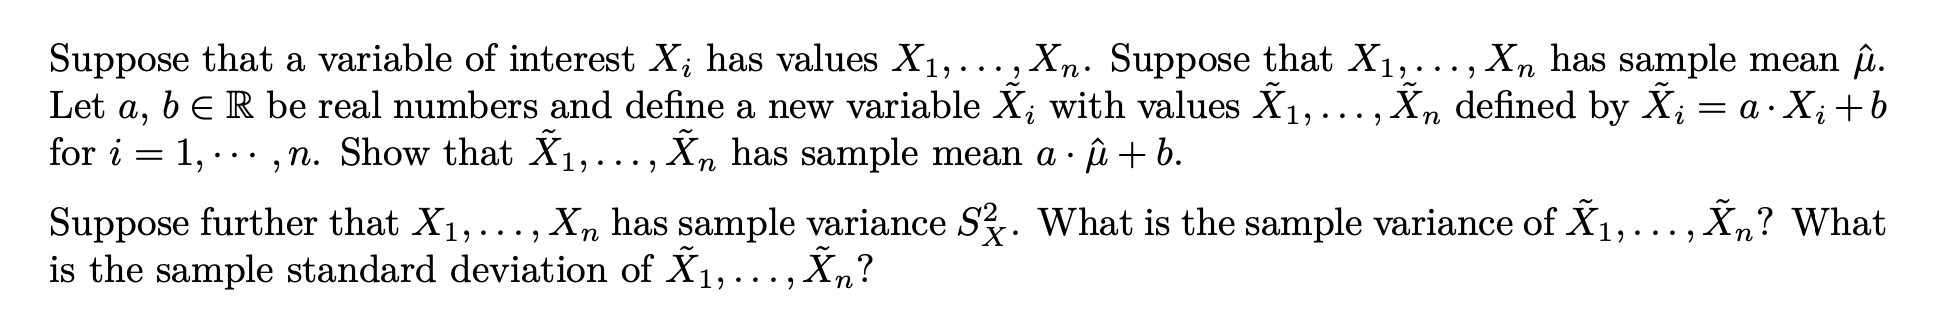
\includegraphics{/Users/frankhu/Documents/SCEM/firstRProject/img/2-3.2.png}
\[\hat\mu=a\mu, \hat{Var}=a^2Var\]

\hypertarget{robustness-of-location-estimators}{%
\subsubsection{3.3 Robustness of location
estimators}\label{robustness-of-location-estimators}}

In this exercise we shall investigate the robustness of several location
estimators: The sample mean, sample median and trimmed mean.

We begin by extracting a vector called ``hal'' consisting of the talon
lengths of all the hawks with any missing values removed.

\begin{Shaded}
\begin{Highlighting}[]
\NormalTok{hal}\OtherTok{\textless{}{-}}\NormalTok{Hawks}\SpecialCharTok{$}\NormalTok{Hallux }\CommentTok{\# Extract the vector of hallux lengths}
\NormalTok{hal}\OtherTok{\textless{}{-}}\NormalTok{hal[}\SpecialCharTok{!}\FunctionTok{is.na}\NormalTok{(hal)] }\CommentTok{\# Remove any nans}
\end{Highlighting}
\end{Shaded}

To investigate the effect of outliers on estimates of location we
generate a new vector called ``corrupted\_hall'' with 10 outliers each
of value 100 created as follows:

\begin{Shaded}
\begin{Highlighting}[]
\NormalTok{outlier\_val}\OtherTok{\textless{}{-}}\DecValTok{100}
\NormalTok{num\_outliers}\OtherTok{\textless{}{-}}\DecValTok{10}
\NormalTok{corrupted\_hal}\OtherTok{\textless{}{-}}\FunctionTok{c}\NormalTok{(hal,}\FunctionTok{rep}\NormalTok{(outlier\_val,}\AttributeTok{times=}\NormalTok{num\_outliers))}
\end{Highlighting}
\end{Shaded}

We can then compute the mean of the original sample and the corrupted
sample as follows.

\begin{Shaded}
\begin{Highlighting}[]
\FunctionTok{mean}\NormalTok{(hal)}
\end{Highlighting}
\end{Shaded}

\begin{verbatim}
## [1] 26.41086
\end{verbatim}

\begin{Shaded}
\begin{Highlighting}[]
\FunctionTok{mean}\NormalTok{(corrupted\_hal)}
\end{Highlighting}
\end{Shaded}

\begin{verbatim}
## [1] 27.21776
\end{verbatim}

Now let's investigate what happens as the number of outliers changes
from 0 to 1000. The code below generates a vector called ``means\_vect''
which gives the sample means of corrupted samples with different numbers
of outliers. More precisely, means\_vect is a vector of length 1001 with
the i-th entry equal to the mean of a sample with i − 1 outliers.

\begin{Shaded}
\begin{Highlighting}[]
\NormalTok{num\_outliers\_vect}\OtherTok{\textless{}{-}}\FunctionTok{seq}\NormalTok{(}\DecValTok{0}\NormalTok{,}\DecValTok{1000}\NormalTok{)}
\NormalTok{means\_vect}\OtherTok{\textless{}{-}}\FunctionTok{c}\NormalTok{()}

\ControlFlowTok{for}\NormalTok{(num\_outliers }\ControlFlowTok{in}\NormalTok{ num\_outliers\_vect)\{}
\NormalTok{  corrupted\_hal}\OtherTok{\textless{}{-}}\FunctionTok{c}\NormalTok{(hal,}\FunctionTok{rep}\NormalTok{(outlier\_val,}\AttributeTok{times=}\NormalTok{num\_outliers))}
\NormalTok{  means\_vect}\OtherTok{\textless{}{-}}\FunctionTok{c}\NormalTok{(means\_vect,}\FunctionTok{mean}\NormalTok{(corrupted\_hal))}
\NormalTok{\}}

\FunctionTok{length}\NormalTok{(means\_vect)}
\end{Highlighting}
\end{Shaded}

\begin{verbatim}
## [1] 1001
\end{verbatim}

Copy and modify the above code to create an additional vector called
``medians\_vect'' of length 1001 with the i-th entry equal to the median
of a sample ``corrupted\_hal'' with i − 1 outliers.

\begin{Shaded}
\begin{Highlighting}[]
\NormalTok{medians\_vect }\OtherTok{\textless{}{-}} \FunctionTok{c}\NormalTok{()}

\ControlFlowTok{for}\NormalTok{(num\_outliers }\ControlFlowTok{in}\NormalTok{ num\_outliers\_vect) \{}
\NormalTok{  corrupted\_hal }\OtherTok{\textless{}{-}} \FunctionTok{c}\NormalTok{(hal, }\FunctionTok{rep}\NormalTok{(outlier\_val, }\AttributeTok{times=}\NormalTok{num\_outliers))}
\NormalTok{  medians\_vect }\OtherTok{\textless{}{-}} \FunctionTok{c}\NormalTok{(medians\_vect, }\FunctionTok{median}\NormalTok{(corrupted\_hal))}
\NormalTok{\}}

\FunctionTok{length}\NormalTok{(medians\_vect)}
\end{Highlighting}
\end{Shaded}

\begin{verbatim}
## [1] 1001
\end{verbatim}

Amend the code further to add an additional vector called
``t\_means\_vect'' of length 1001 with the i-th entry equal to the
trimmed mean of a sample with i−1 outliers, where the trimmed mean has a
trim fraction q = 0.1.

\begin{Shaded}
\begin{Highlighting}[]
\NormalTok{t\_means\_vect }\OtherTok{\textless{}{-}} \FunctionTok{c}\NormalTok{()}

\ControlFlowTok{for}\NormalTok{(num\_outliers }\ControlFlowTok{in}\NormalTok{ num\_outliers\_vect) \{}
\NormalTok{  corrupted\_hal }\OtherTok{\textless{}{-}} \FunctionTok{c}\NormalTok{(hal, }\FunctionTok{rep}\NormalTok{(outlier\_val, }\AttributeTok{times=}\NormalTok{num\_outliers))}
\NormalTok{  t\_means\_vect }\OtherTok{\textless{}{-}} \FunctionTok{c}\NormalTok{(t\_means\_vect, }\FunctionTok{mean}\NormalTok{(corrupted\_hal, }\AttributeTok{trim =} \FloatTok{0.1}\NormalTok{))}
\NormalTok{\}}

\FunctionTok{length}\NormalTok{(t\_means\_vect)}
\end{Highlighting}
\end{Shaded}

\begin{verbatim}
## [1] 1001
\end{verbatim}

You should now have four vectors: ``num\_outliers\_vect'',
``means\_vect'', ``medians\_vect'' and ``t\_means\_vect''. Combine these
vectors into a data frame with the following code.

\begin{Shaded}
\begin{Highlighting}[]
\NormalTok{df\_means\_medians }\OtherTok{\textless{}{-}} \FunctionTok{data.frame}\NormalTok{(}\AttributeTok{num\_outliers=}\NormalTok{num\_outliers\_vect,}\AttributeTok{mean=}\NormalTok{means\_vect,}\AttributeTok{t\_mean=}\NormalTok{t\_means\_vect,}\AttributeTok{median=}\NormalTok{medians\_vect)}
\end{Highlighting}
\end{Shaded}

Now use the code below to reshape and plot the data. The function
pivot\_longer() below is used to reshape the data. Don't worry if this
operation is unclear at this stage. Its use will be explained soon.

\begin{Shaded}
\begin{Highlighting}[]
\NormalTok{df\_means\_medians}\SpecialCharTok{\%\textgreater{}\%}
  \FunctionTok{pivot\_longer}\NormalTok{(}\SpecialCharTok{!}\NormalTok{num\_outliers, }\AttributeTok{names\_to =} \StringTok{"Estimator"}\NormalTok{, }\AttributeTok{values\_to =} \StringTok{"Value"}\NormalTok{)}\SpecialCharTok{\%\textgreater{}\%}
  \FunctionTok{ggplot}\NormalTok{(}\FunctionTok{aes}\NormalTok{(}\AttributeTok{x=}\NormalTok{num\_outliers,}\AttributeTok{color=}\NormalTok{Estimator,}\AttributeTok{linetype=}\NormalTok{Estimator,}\AttributeTok{y=}\NormalTok{Value))}\SpecialCharTok{+}
  \FunctionTok{geom\_line}\NormalTok{()}\SpecialCharTok{+}\FunctionTok{xlab}\NormalTok{(}\StringTok{"Number of outliers"}\NormalTok{)}
\end{Highlighting}
\end{Shaded}

\includegraphics{Assignment2Notebook_files/figure-latex/unnamed-chunk-32-1.pdf}
\#\#\# 3.4 Box plots and outliers

Use the functions ggplot() and geom\_boxplot() to create a box plot
which summarises the distribution of hawk weights broken down by
species.

\begin{Shaded}
\begin{Highlighting}[]
\FunctionTok{ggplot}\NormalTok{(Hawks, }\FunctionTok{aes}\NormalTok{(Species, Weight)) }\SpecialCharTok{+} \FunctionTok{geom\_boxplot}\NormalTok{()}
\end{Highlighting}
\end{Shaded}

\begin{verbatim}
## Warning: Removed 10 rows containing non-finite values (stat_boxplot).
\end{verbatim}

\includegraphics{Assignment2Notebook_files/figure-latex/unnamed-chunk-33-1.pdf}

Suppose we have a sample X1, · · · , Xn. Let q25 denote the
0.25-quantile of the sample and let q75 denote the 0.75-quantile of the
sample. We can then define the interquartile range, denoted IQR by
\texttt{IQR\ :=\ q75\ −\ q25}. In the context of boxplots and outlier Xi
is any numerical value such that the following holds if either of the
following holds:\\
\[X_i < q25 - 1.5 \times IQR\] \[X_i > q75 + 1.5 \times IQR\]

Create a function called ``num\_outliers'' which computes the number of
outliers within a sample (with missing values excluded).

Now combine your function num\_outliers() with the functions
\texttt{group\_by()} and \texttt{summarise()} to com- pute the number of
outlier for the three samples of hawk weights broken down by specied.

\begin{Shaded}
\begin{Highlighting}[]
\CommentTok{\# num\_outliers \textless{}{-} function(.data, feature) \{}
\CommentTok{\#   q25 \textless{}{-}quantile(.data[feature], 0.25, na.rm=TRUE)}
\CommentTok{\#   q75 \textless{}{-}quantile(.data[feature], 0.75, na.rm=TRUE)}
\CommentTok{\#   iq\_range \textless{}{-} q75 {-} q25}
\CommentTok{\#   outliers \textless{}{-} .data[feature][feature \textgreater{} q75+1.5*iq\_range | feature \textless{} q25{-}1.5*iq\_range | is.na(feature)]}
\CommentTok{\#   return (sum(is.na(.data[feature]))+nrow(outliers))}
\CommentTok{\# \}}


\NormalTok{num\_outliers }\OtherTok{\textless{}{-}} \ControlFlowTok{function}\NormalTok{(feature) \{}
\NormalTok{  q25 }\OtherTok{\textless{}{-}}\FunctionTok{quantile}\NormalTok{(feature, }\FloatTok{0.25}\NormalTok{, }\AttributeTok{na.rm=}\ConstantTok{TRUE}\NormalTok{)}
\NormalTok{  q75 }\OtherTok{\textless{}{-}}\FunctionTok{quantile}\NormalTok{(feature, }\FloatTok{0.75}\NormalTok{, }\AttributeTok{na.rm=}\ConstantTok{TRUE}\NormalTok{)}
\NormalTok{  iq\_range }\OtherTok{\textless{}{-}}\NormalTok{ q75 }\SpecialCharTok{{-}}\NormalTok{ q25}
\NormalTok{  outliers }\OtherTok{\textless{}{-}}\NormalTok{ feature[feature }\SpecialCharTok{\textgreater{}}\NormalTok{ q75}\FloatTok{+1.5}\SpecialCharTok{*}\NormalTok{iq\_range }\SpecialCharTok{|}\NormalTok{ feature }\SpecialCharTok{\textless{}}\NormalTok{ q25}\FloatTok{{-}1.5}\SpecialCharTok{*}\NormalTok{iq\_range ]}
  \FunctionTok{return}\NormalTok{ (}\FunctionTok{sum}\NormalTok{(}\FunctionTok{is.na}\NormalTok{(feature))}\SpecialCharTok{+}\FunctionTok{length}\NormalTok{(outliers))}
\NormalTok{\}}
\end{Highlighting}
\end{Shaded}

\begin{Shaded}
\begin{Highlighting}[]
\NormalTok{ch\_hawks }\OtherTok{\textless{}{-}}\NormalTok{ Hawks }\SpecialCharTok{\%\textgreater{}\%} \FunctionTok{filter}\NormalTok{(Species}\SpecialCharTok{==}\StringTok{"CH"}\NormalTok{)}
\NormalTok{ch\_weight }\OtherTok{\textless{}{-}}\NormalTok{ ch\_hawks[}\StringTok{"Weight"}\NormalTok{]}

\NormalTok{q25 }\OtherTok{\textless{}{-}} \FunctionTok{quantile}\NormalTok{(ch\_weight, }\FloatTok{0.25}\NormalTok{, }\AttributeTok{na.rm=}\ConstantTok{TRUE}\NormalTok{)}
\NormalTok{q75 }\OtherTok{\textless{}{-}} \FunctionTok{quantile}\NormalTok{(ch\_weight, }\FloatTok{0.75}\NormalTok{, }\AttributeTok{na.rm=}\ConstantTok{TRUE}\NormalTok{)}
\NormalTok{iq\_range }\OtherTok{\textless{}{-}}\NormalTok{ q75 }\SpecialCharTok{{-}}\NormalTok{ q25}
\NormalTok{outliers }\OtherTok{\textless{}{-}}\NormalTok{ ch\_weight[ch\_weight }\SpecialCharTok{\textless{}}\NormalTok{ q25}\FloatTok{{-}1.5}\SpecialCharTok{*}\NormalTok{iq\_range }\SpecialCharTok{|}\NormalTok{ ch\_weight }\SpecialCharTok{\textgreater{}}\NormalTok{ q75}\FloatTok{+1.5}\SpecialCharTok{*}\NormalTok{iq\_range]}
\end{Highlighting}
\end{Shaded}

\begin{Shaded}
\begin{Highlighting}[]
\NormalTok{Hawks }\SpecialCharTok{\%\textgreater{}\%} \FunctionTok{group\_by}\NormalTok{(Species) }\SpecialCharTok{\%\textgreater{}\%} \FunctionTok{summarise}\NormalTok{(}\AttributeTok{num\_outliers\_weight=}\FunctionTok{num\_outliers}\NormalTok{(Weight))}
\end{Highlighting}
\end{Shaded}

\begin{verbatim}
## # A tibble: 3 x 2
##   Species num_outliers_weight
##   <fct>                 <int>
## 1 CH                        3
## 2 RT                       23
## 3 SS                       14
\end{verbatim}

\hypertarget{covariance-and-correlation-under-linear-transformations}{%
\subsubsection{3.5 Covariance and correlation under linear
transformations}\label{covariance-and-correlation-under-linear-transformations}}

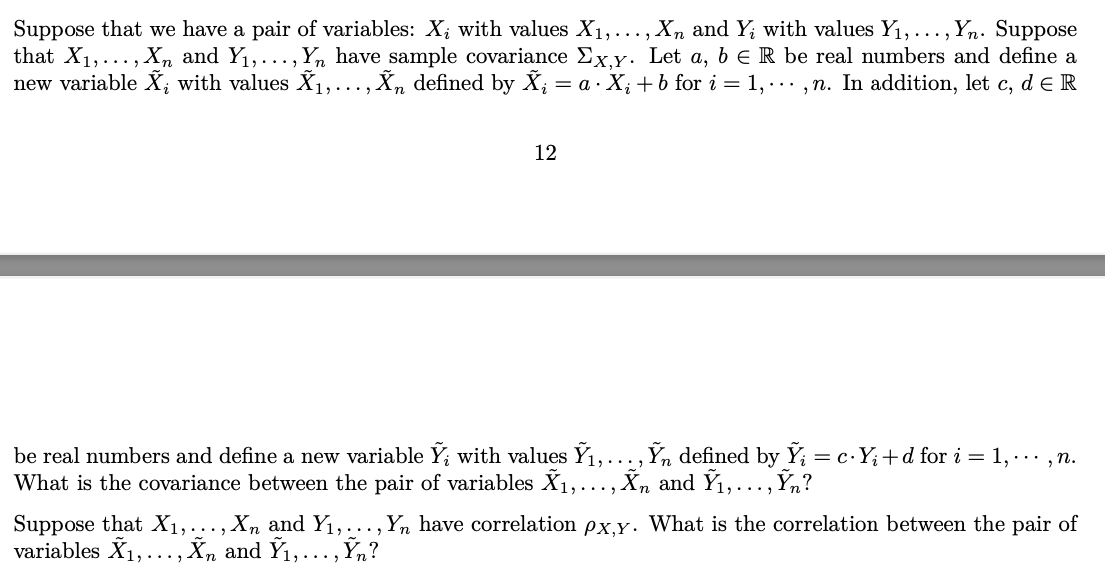
\includegraphics{/Users/frankhu/Documents/SCEM/firstRProject/img/2-3.5.png}
\textbf{Answer:} \(\hat\rho_{X, Y}=a^2\rho_{X,Y}\)

\end{document}
